\section{A historical perspective on bioinformatics}
Many decades ago, around the 1950s, we did not know much about the molecules that carry our genetic information and how this would be translated into higher levels of biology. All that was known about deoxyribonucleic acid (DNA) was that it carries nucleotides in equimolar proportions so that there is as much guanine as cytodine and as much adenine as thymine. A major breakthrough came with Watson and Crick's discovery of the structure of DNA in 1953~\cite{dnastruct}. Despite that, it took some more decades before the genetic code was deciphered and how this information is further transferred. Researchers came to know that DNA is essentially built up of a linear sequence of the four aforementioned nucleic acids. This sequence encodes information that undergoes transcription into ribonucleic acid (RNA) that in turn gets translated into proteins. The encoding of proteins is done in groups of three nucleic acids at a time, known as codons. All of this was later stated as the \textit{central dogma of molecular biology}, also by Crick in 1958~\cite{dogma}. This was hugely important for later research since it gives us more insight into how the genetic code is translated and transferred.
\begin{figure}[h]
    \centering
    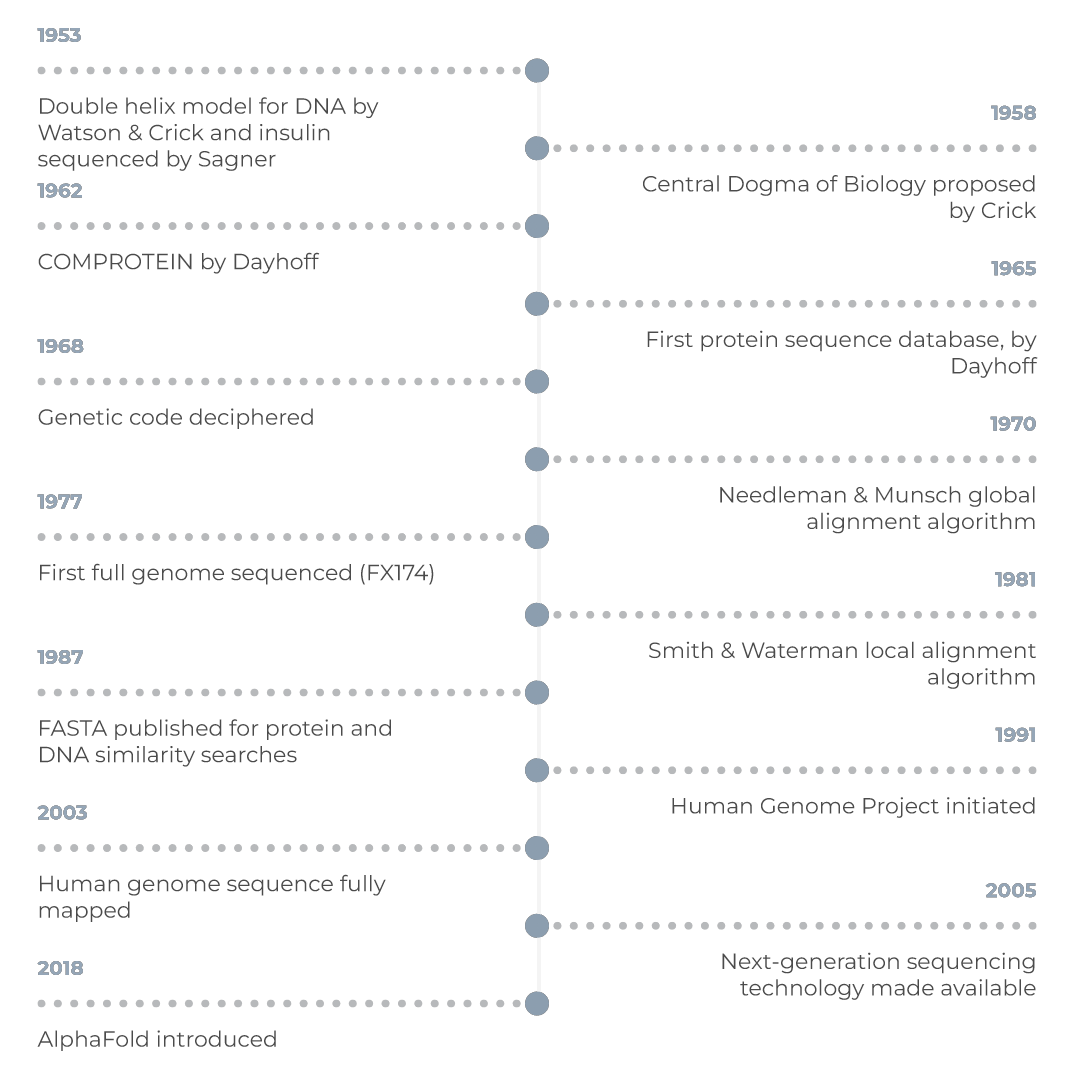
\includegraphics[scale = 0.5]{timeline.png}
    \caption{A brief timeline of important developments in bioinformatics.}
    \label{fig:timeline}
\end{figure}
In the same decade, major leaps were made in the research of protein structure and sequences. The first three-dimensional protein structures were determined via X-ray crystallography~\cite{xray}, which is still mostly the preferred method to this day. On top of that, the arrangement of the primary structure of a protein has been resolved after the first sequencing of a polypeptide. Sanger determined by sequencing insulin in 1953~\cite{insulin} that a protein is built up of a sequence of amino acids, all connected by a peptide bond into a polypeptide. This established the idea that proteins are biological macromolecules that carry lots of information~\cite{primstruct}, which started a boom of research on more efficient methods for obtaining protein sequences. The most popular method of that time was the Edman degradation method~\cite{edman}. A major issue with this method was that only a theoretical maximum of 50 to 60 sequential amino acids could be sequenced. Larger proteins had to be cleaved into fragments that were small enough to be sequenced. Tracing back the input sequence from this data was a cumbersome process and thus published Dayhoff the first computational program applied to biological data, COMPROTEIN~\cite{comprotein} in 1962. This program was essentially a \textit{de novo} sequence assembler for Edman degradation data. Furthermore, sequencing amino acids was also increasingly made automated later in the 1960s. These innovations assisted the creation of the first published protein sequence database~\cite{atlas} in 1965.

Further in the 1960s, researchers discovered the evolutionary value of having protein sequence data of different species. The problem to be solved back then was the quantification of the similarity between sequences. Pairwise alignment algorithms such as the algorithm of Needleman \& Wunsch~\cite{global} for global alignments and that of Smith \& Waterman~\cite{local} for local alignments from the 1970s solved this issue and alignment is still considered to be a key bioinformatics task to this day. Together with this, mathematical frameworks for amino acid substitutions in the context of evolution such as PAMs and BLOSUMs also contributed to bioinformatics. These pairwise alignment algorithms are sufficient for comparing two sequences but unfeasible for searching databases for homologous sequences, hence faster algorithms like FASTA~\cite{fasta}, BLAST~\cite{blast} were developed in the 1980s and 1990s. These methods were and are still important for discovering functional, structural and evolutionary information in biological sequences since sequences that are in some way similar, have a high chance to have the same biological function. This also means that such sequences might be derived from a common ancestor and it became commonplace that sequence patterns may lead to structural and functional relevance. A natural extension of pairwise alignments is multiple sequence alignment (MSA)~\cite{msa}, which is to align multiple related sequences. The most popular and still widely used tools today include Clustal~\cite{clustal} and MUSCLE~\cite{muscle}. This reveals much more information than pairwise alignment can. It allows for the identification of conserved sequence patterns and critical amino acid residues with much more statistical significance which is of great value for constructing phylogenetic profiles of gene families~\cite{phylo}. All of this showed the importance of computational biology and established bioinformatics as a beneficial field of science.

Development of DNA-based applications took some more time since the genetic code and how it translates to amino acids was not deciphered yet until 1968~\cite{codon}. Early DNA and RNA sequencing methods were first demonstrated in the 1970s~\cite{dnaseq, rna} and like with protein sequencing methods, these methods only became faster, more efficient and more scalable. The 1990s saw the appearance of whole genome sequencing and internet-accessible databases that we still use to this day, such as Genbank, Genomes and PubMed and so advances in computational biology followed the ever-increasing amount of data and need for processing power. With the advent of second-generation sequencing in the 2000s came even more Big Data issues, further challenging bioinformaticians by allowing us to sequence millions of DNA and RNA molecules in a single run. The sheer size and complexity of biological data can make it difficult to store and manage, as for instance implementing error identification, security, quality standards and easy data retrievability. On top of that, the analysis of such large-scale data is not straightforward and traditional software tools won't be sufficient anymore. Lastly, the need for high-performance computing resources to handle all of these computational demands will only rise.

Today we see that research in the field of biology is becoming more and more computationally driven and that this trend will not slow down any time soon. As for this thesis, we will focus on this matter, more specifically on the level of protein research which is discussed in the next section.